\documentclass[Master.tex]{subfiles}
\begin{document}

\begin{frame}
	\begin{figure}
\centering

\includegraphics[width=0.7\linewidth]{images/DeepLearningUseless}
\caption{}
\label{fig:DeepLearningUseless}
\end{figure}

\end{frame}	
\begin{frame}
	\frametitle{Statistics with Julia}
	\Large
	\begin{quote}
		``.....Can he do it on a cold, wet Wednesday night in Stoke?"
	\end{quote}
\end{frame}
\begin{frame}
	\frametitle{Statistics with Julia}
	\large
	\begin{description}
		\item[1st Year]	Exploratory Data Analysis,	Summary Statistics, Probability, Graphical Methods \smallskip
		\item[2nd Year]	Hypothesis Testing, Confidence Intervals, Probability Distributions, Linear Models \smallskip
		\item[3rd Year] ANOVA and Experimental Design, Residuals, Chi Squared, Stepwise Regression \smallskip
		\item[4th Year] PCA, Clustering, Logistic Regression
	\end{description}
\end{frame}	
%======================================================%
\begin{frame}
	\frametitle{Statistics with Julia}
	\large
		\textbf{What is like to teach statistics }vs \textbf{What it should be like} \\ \smallskip
		
		
		The Future according to Kevin
	\begin{itemize}
		\item Remove Pen and Paper Calculations\\ \textit{(Keep a few good ones)}
		
		\item Sort out Bad Instructional Design \\ \textit{(time is short...dont waste time with stupid crap)}
		
		\item Why the flip is this still an exam question? Is this still the 30s?
		
		\item (The t-test is actually fairly robust to non-normality).
		
		\item e.g. Sum of Squares Identities in Experimental Design..\textbf{BY HAND...F.R.O!!!}
	\end{itemize}

\end{frame}	

%======================================================%
\begin{frame}
	\frametitle{Statistics with Julia}
	\large
	\textbf{Writing Stats Exams!!}
	\begin{itemize}
		\item Copy and Paste questions some past papers 
		\item change a few numbers here and there
		\item Transforms weights of dogs into heights of cats
		\[ X  \sim {1000,25^2} \]
		\item Why fix that equation? too much like work?
		
	\end{itemize}	
	\textbf{Exam papers take time....	Hey, you got better things to do!!!}
	
\end{frame}	
\begin{frame}
	\begin{figure}
\centering
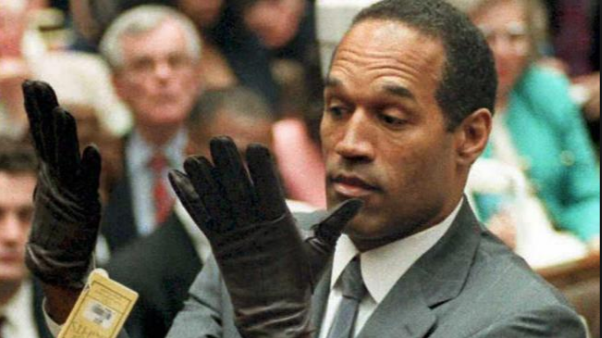
\includegraphics[width=0.98\linewidth]{images/OJ}
\end{figure}

\end{frame}
\begin{frame}
	\frametitle{Statistics with Julia}
	\large	
Hypothesis Testing it a bit like a trial

\begin{description}	
\item[Ho :] Innocent
\item[H1 :] Guilty
\end{description}	
	Got enough evidence to convict? Reasonable doubt
\end{frame}
%====================================================%
\begin{frame}
	\frametitle{Statistics with Julia}
	\large	
	\begin{itemize}
		\item Put in more p-values...but learning to critique the analysss proplerly
		
		\item Tell them about P-hacking
		
		\item and anyway...What exactly is a confidence interval (for mean?)
	\end{itemize}

\end{frame}

\begin{frame}
	\begin{figure}
\centering
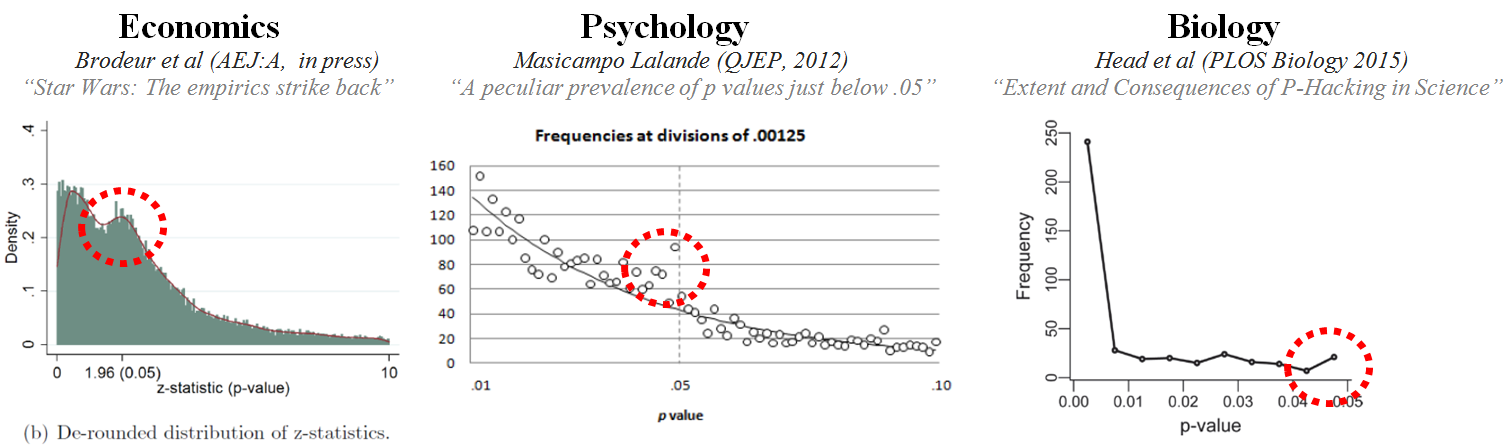
\includegraphics[width=1.1\linewidth]{images/phacking}
\caption{}
\label{fig:phacking}
\end{figure}

\end{frame}	
%======================================================%
\begin{frame}
	\frametitle{Statistics with Julia}
	\large
	\begin{itemize}
	\item Never omit "Type I" Error and "Type II" Error
	
	\item HT is not about what is true or false it is above what you can prove (back up with a sufficient amount of evidence)
	
	\item You'd be surprised about how many people dont know that.
	\end{itemize}
\end{frame}

\begin{frame}
	
	\begin{figure}
\centering

\includegraphics[width=0.99\linewidth]{images/AutomateAllTheThings}

\end{figure}

\end{frame}	
\begin{frame}
\begin{figure}
\centering

\includegraphics[width=0.99\linewidth]{images/JupyterCloud}
\caption{}
\label{fig:JupyterCloud}
\end{figure}


\end{frame}

\begin{frame}
	\begin{figure}
\centering
\includegraphics[width=0.98\linewidth]{images/JuliaBox}
\caption{}
\label{fig:JuliaBox}
\end{figure}

\end{frame}
%======================================================%
\begin{frame}
	\frametitle{Statistics with Julia}
	\large
	
	Surely students could handle some code?
	
	\begin{itemize}
		\item \texttt{sample()}
		\item \texttt{mean()}
		\item \texttt{t.test()}
		
	\end{itemize}
	
	They dont have to like it, but they would prefer having to do some basic computing as opposed to.....
\end{frame}	
%======================================================%
\begin{frame}
	\frametitle{Statistics with Julia}
	\large
	\begin{figure}
\centering
\includegraphics[width=0.99\linewidth]{"C:/Users/Computer Six/Documents/GitHub/JuliaWorkshop.github.io/00-StatisticsWithJulia/images/SS"}
\end{figure}

2 Hours of my life wasted!!!\\
\textit{(Although some are worth keeping)}

\end{frame}	
%======================================================%
\begin{frame}
\frametitle{Statistics with Julia}
\large
\textbf{Non-parametric statistics}
		
\begin{itemize}		
\item ranked data
\item Likert scale
\item \textbf{carrying out a heart transplant with a shovel}
\item hard to prove anything to satisfactory degree
\end{itemize}
\end{frame}
%======================================================%
\begin{frame}
	\frametitle{Statistics with Julia}
	\large
\begin{figure}
\centering
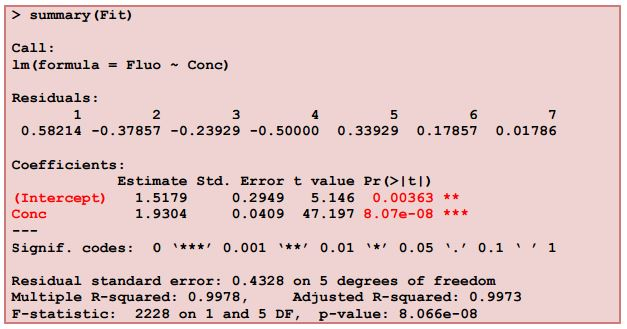
\includegraphics[width=1.1\linewidth]{images/LoD}
\caption{}
\label{fig:LoD}
\end{figure}

\end{frame}
\begin{frame}
	\frametitle{Statistics with Julia}
	\large
This is \texttt{R}, but same argument applies to Julia.	
\begin{itemize}
\item \texttt{AIC()}
\item \texttt{summary()}
\item \texttt{cor.test()}
\item \texttt{plot(Fit)}
\end{itemize}
\end{frame}	

%=====================================================%
\begin{frame}[fragile]
	\begin{verbatim}
	julia> # Pkg.clone("git://github.com/JuliaQuant/MarketData.jl.git") # brings in TimeSeries package too
	
	julia> using MarketData, Gadfly, HypothesisTests
	
	julia> dist = percentchange(cl).values;
	
	julia> funkydist = dist[100:300];
	
	julia> SignTest(funkydist)
	Sign test
	
	median = 0.0
	x = 111
	n = 201
	
	Two-sided p-value:
	p = 0.15816534520094128
	
	\end{verbatim}
	
\end{frame}

\begin{frame}
\begin{figure}
\centering
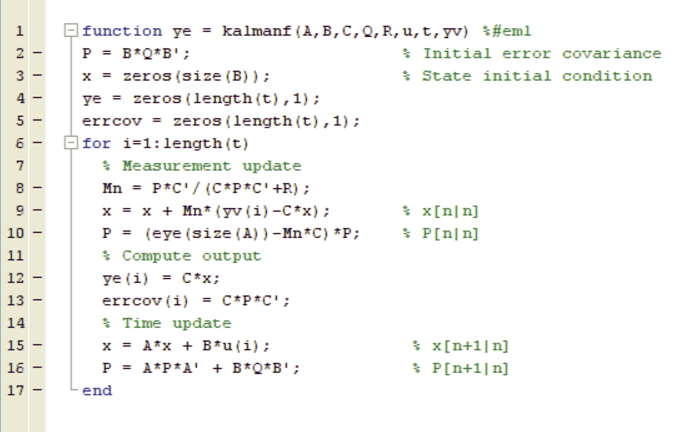
\includegraphics[width=0.9\linewidth]{images/MATLAB}
\caption{}
\label{fig:MATLAB}
\end{figure}
\end{frame}
%==============================================%
\begin{frame}
	\frametitle{Statistics with Julia}
	\large
	
	\begin{itemize}
		\item StatsBase
		\item DataFrames
		\item RDatasets
	\end{itemize}
	
\end{frame}	
%=========================================================%
%==============================================%
\begin{frame}[fragile]
	\large
\begin{itemize}
\item Stuff that gets me 
	
\item I still think in "R", not MATLAB
	
\item Why is this not working (in Julia)?
\end{itemize}	


\begin{verbatim}
myData[myData < 400]
\end{verbatim}
If I thought in MATLAB, Julia is fairly easy to pick up

\end{frame}
\begin{frame}
	\begin{figure}
\centering
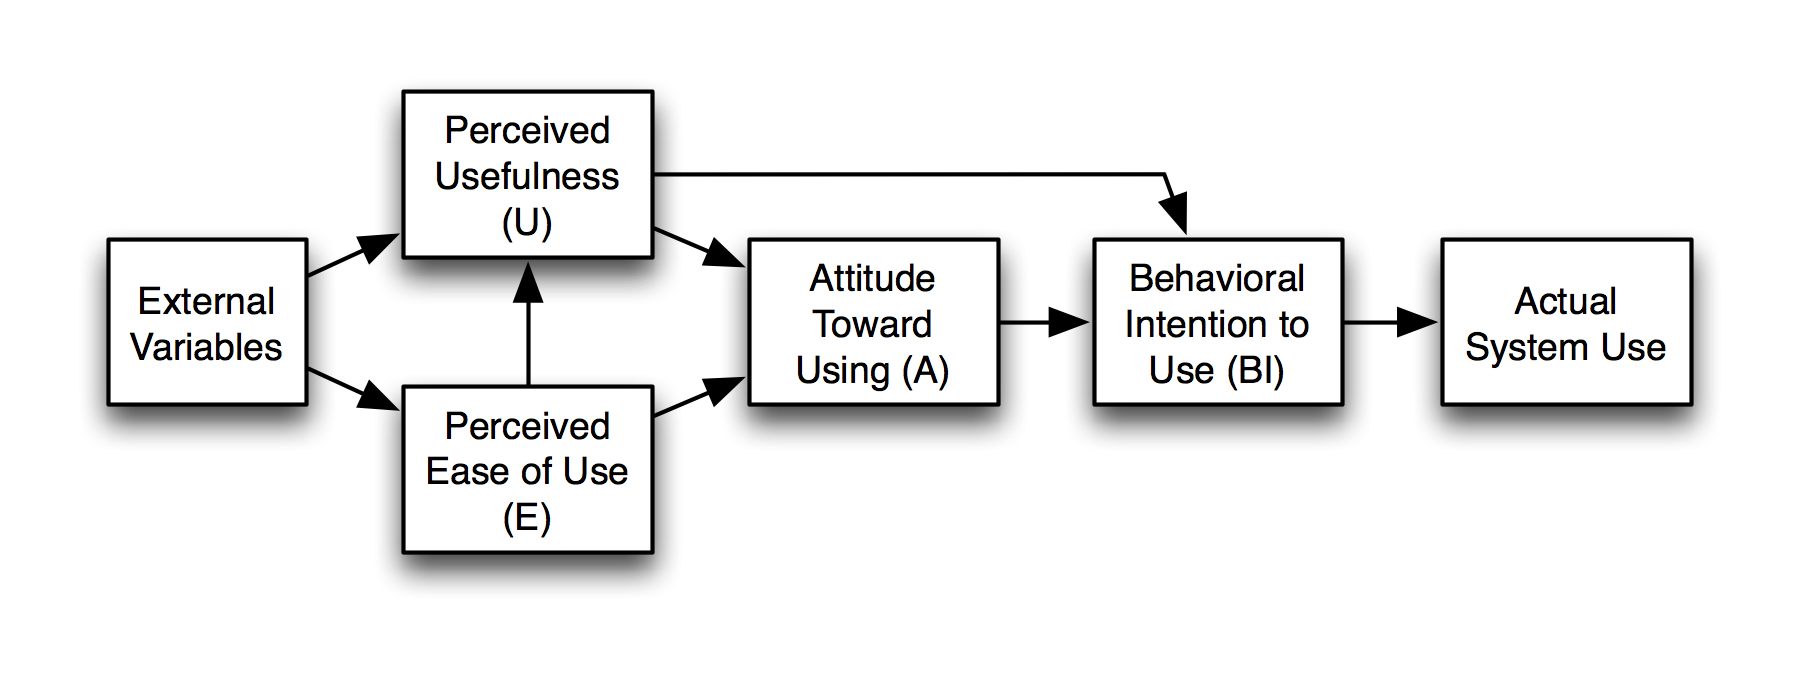
\includegraphics[width=0.7\linewidth]{images/Technology_Acceptance_Model}
\caption{}
\label{fig:Technology_Acceptance_Model}
\end{figure}
\end{frame}


\end{document}